\documentclass[12pt]{article}
\usepackage{algos-tasks}

\usepackage{graphicx}
\graphicspath{{draw-tree-assets/}}

\newcommand{\todo}{$\blacktriangleright$\quad}

\begin{document}
\task[latex]{Growing Trees with \TikZ}

\TikZ{} is a language for drawing graphics that can be used within \LaTeX.

In this task, we'll use \TikZ{} to draw a tree. It should look something like this:

\begin{center}
    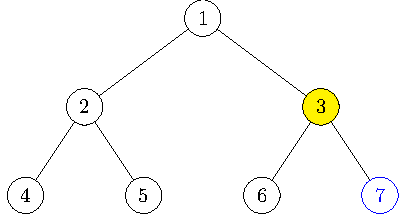
\includegraphics[width=0.5\linewidth]{draw_tree.pdf}
\end{center}
    

\todo Steps for you to do are marked with a triangle.

\subsection*{Setting up}
\todo To start, create a new \emph{standalone} document in a \verb|.tex| file:

\begin{lstlisting}
\documentclass{standalone}
\begin{document}

\end{document}
\end{lstlisting}

This document class provides only the bare necessities to make an image, and crops the resulting page.

\todo You may recall from \textit{`Hello, World!'} in Module 1 that the section before \verb|\begin{document}| is called the \emph{preamble}, and is where we put configuration options. This time, we will add a command to import the \TikZ{} package. Add this line to your preamble:

\begin{lstlisting}
\usepackage{tikz}
\end{lstlisting}

You can think of this like a \verb|#include| in C.

\subsection*{Drawing a picture}
\todo To create our picture, we first need to open a \verb|tikzpicture| environment. Use \verb|\begin| and \verb|\end| to create the environment, and put the following code inside:

\begin{lstlisting}
\draw[fill=blue!40!white] (0,0) -- (4,0) -- (4,4) -- (0,4) -- (0,0);
\end{lstlisting}

Compile your document and see what you get!

\todo To learn more about the basics of \TikZ{}, follow \href{https://www.overleaf.com/learn/latex/LaTeX_Graphics_using_TikZ\%3A_A_Tutorial_for_Beginners_(Part_1)%E2%80%94Basic_Drawing}{this} tutorial.

\subsection*{Nodes and Edges}

In \TikZ, a node is simply some text at a point. For example,
\begin{lstlisting}
\node (a) at (0, 0) {Hello! $2 + 2 = 4$};
\end{lstlisting}

The \verb|(a)| is the name of the node, and will not be drawn. We can use this to refer to the node later:

\begin{lstlisting}
\node at (0, 0) {Hello! $2 + 2 = 4$};
\node (b) [below=1cm of a] {Hi! $3 + 3 = 6$};
\end{lstlisting}

The node name can be left out if we don't need it. We'll look closer at nodes when we draw graphs later. Now, let's make a tree!

\subsection*{Trees}

\todo Start a new standalone document with \TikZ\ included, and place the following code in the body of the document:
\begin{lstlisting}
\begin{tikzpicture}
\node {1}
    child {node {2}}
    child {node {3}};
\end{tikzpicture}
\end{lstlisting}

Here, we've used the \verb|child| operation to give the node containing `1' a left and a right child. Currently, the nodes just show a number - let's give them an outline. As you've seen already, we can put options in square brackets \verb|[]| to specify colours, placements and other properties of the elements in our picture. Multiple options can be separated by commas.

\todo Add the \verb|draw| and \verb|circle| properties to each node to give them a circular outline.

Manually adding options to each node gets tedious when we have a lot of nodes. Instead, we can specify to draw a circle around \textit{every node} in the picture using a style:

\begin{lstlisting}
\begin{tikzpicture}[every node/.style = {draw}]
\end{lstlisting}

\todo Add the style to draw a circular outline around every node.

Now, let's add some more nodes! We want to have 4 and 5 as the child nodes of 2, and 6 and 7 as the children of 3.

\todo Add the nodes 4, 5, 6 and 7.

Unfortunately, nodes 5 and 6 now overlap. To fix this, we will add more styles! As well as applying a style to every node, we can apply a style to a layer using \verb|level x/.style|. Each layer of children gets a level starting from 1, so the root's children are \verb|level 1|, and its grandchildren are \verb|level 2|. Is the root level 0? Try it and find out!

In this case, we want to use the \verb|sibling distance| option. Unlike \verb|draw|, this option takes a numeric value, which we assign with an \verb|=| symbol, e.g. \verb|sibling distance=1|. We can also specify a unit, e.g. \verb|1cm|. 

\todo Use level styles and \verb|sibling distance| to fix the overlapping nodes. 

Finally, we can add some decoration! Just like \verb|sibling distance|, the \verb|fill| option takes a parameter (in this case, a colour). You can also set the text colour by just specifying a colour as a standalone option (e.g. \verb|blue|). Rather than applying this to all the nodes, we want to apply this to individual nodes, so we won't use a style.

\todo Use the fill and colour options to decorate the tree! Do some research and find some other options to style more nodes with.

\bigskip

\begin{question}
Follow the steps given to produce a tree diagram using \TikZ. Submit both the compiled PDF and your \verb|.tex| code.
\end{question}

\begin{rubric}

Produce a tree in \TikZ{} similar to the one shown. In particular,
\begin{itemize}
    \item Nodes numbered 1 to 7 with circular outlines,
    \item No overlapping nodes,
    \item Formatting applied with fill, colour and other style options,
    \item Use of styles for node outlines and level distances.
\end{itemize}
Your \TikZ{} code should be well-formatted and readable, with good use of indentation and spacing.
\end{rubric}
\end{document}
